\section{The Problem}

\begin{frame}
  \frametitle{The Problem: Power Law Graphs are Common}
  \begin{itemize}
      \item An imporant class of natural graphs.
      \item A few \textit{very high-degree vertices}.
      \item Hard to partition.
      \item These vertices cause performance and scalability challenges for
            existing graph-parallel systems.
  \end{itemize}
\end{frame}

\subsection{Some Background on Power Law Graphs}

\begin{frame}
    \textbf{Q:} What's a Power Law Graph?

    \textbf{A:} A graph whose vertex degree distribution is a power law
    distribution.
\end{frame}

\begin{frame}
  \frametitle{Power Law Functions Have A Characteristic Shape}
  \begin{figure}
    \centering
    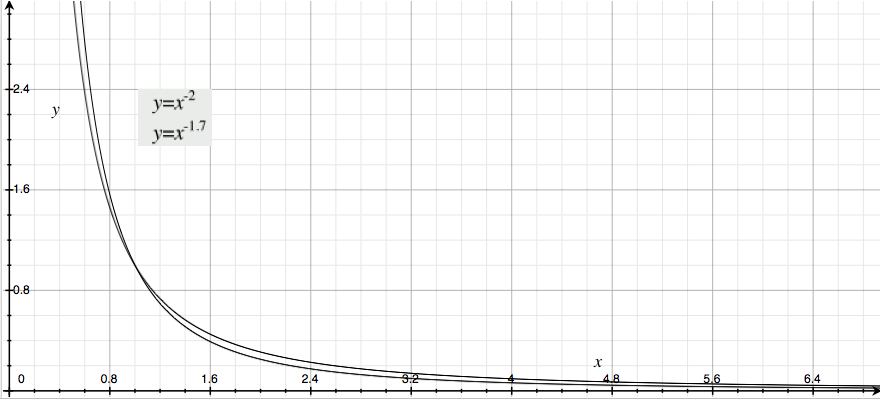
\includegraphics[scale=0.29]{two_power_law_functions}
    \caption{Two power law functions ($\alpha = 1.7$ and $\alpha = 2$) on a
             Cartesian coordinate system. A \textit{power law} is a
             proportionality relation between two values of the form
             $y \propto x^{-\alpha}$, where $\alpha$ is positive. A power law
             \textit{distribution} is just a probability distribution of this
             form.}
  \end{figure}
\end{frame}

\begin{frame}
  \frametitle{Many Natural Graphs Are Power Law Graphs}
  \begin{figure}
    \centering
    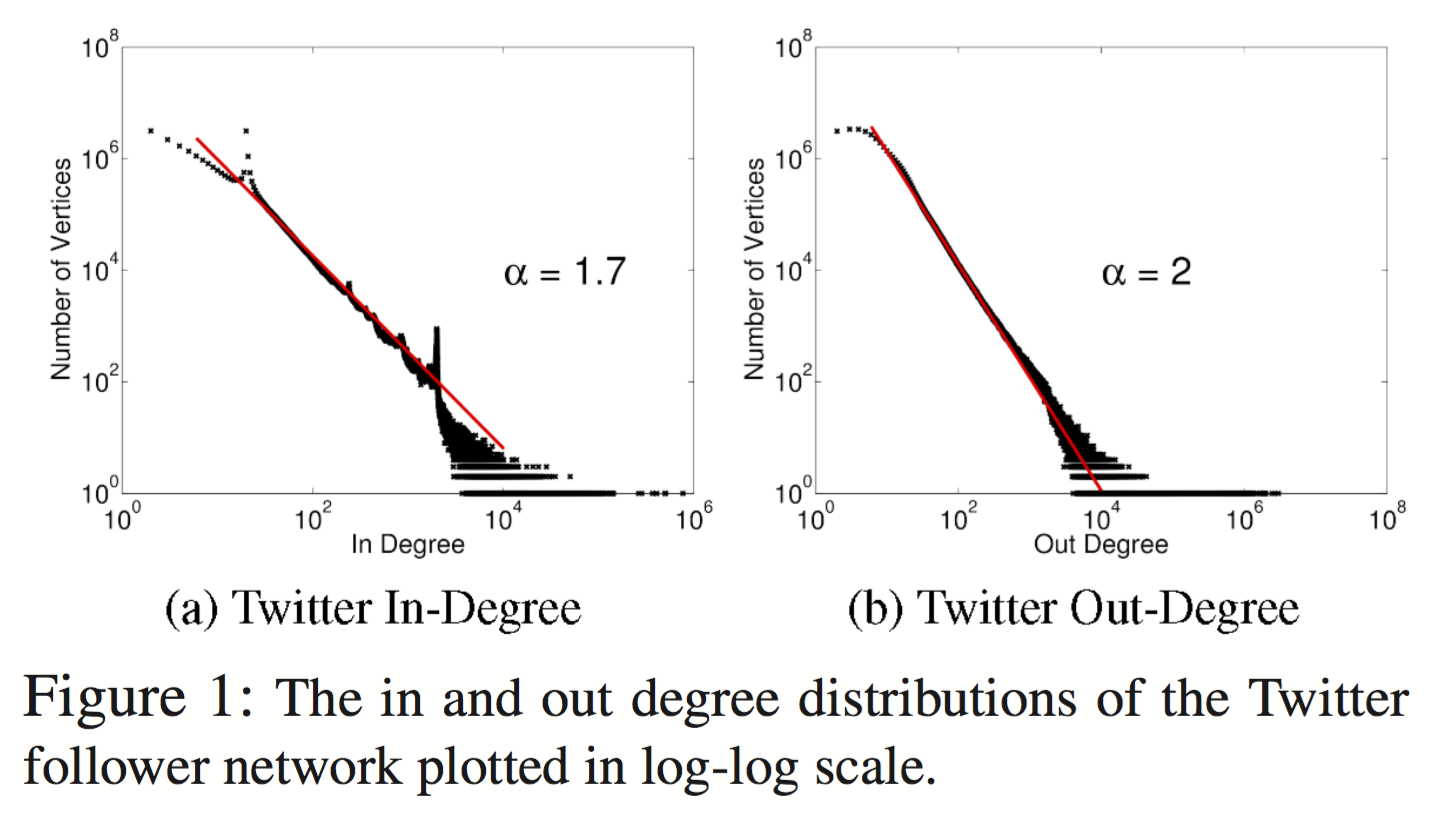
\includegraphics[scale=0.17]{gonzalez_osdi_2012_figure_1}
    \caption{\cite[OSDI '12]{gonzalez2012powergraph}}
  \end{figure}
\end{frame}

\begin{frame}
  \frametitle{A Small Number of Vertices are of Very High Degree}
  \begin{figure}
    \centering
    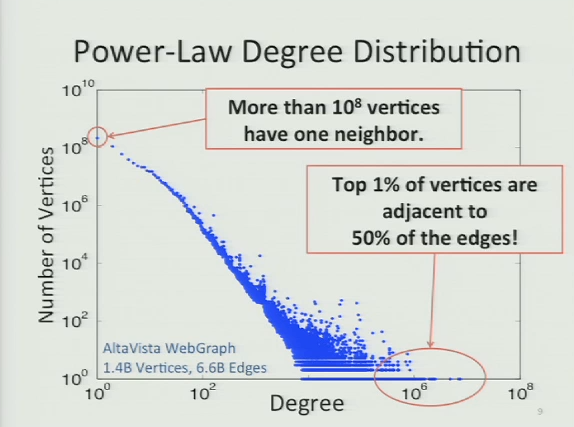
\includegraphics[scale=0.32]{gonzalez_osdi_2012_slide_9}
    \caption{\cite[OSDI '12 Slides]{gonzalez2012powergraph-slides}}
  \end{figure}
\end{frame}

\begin{frame}
  \frametitle{Power Law Graphs Are Hard to Partition}
  \begin{figure}
    \centering
    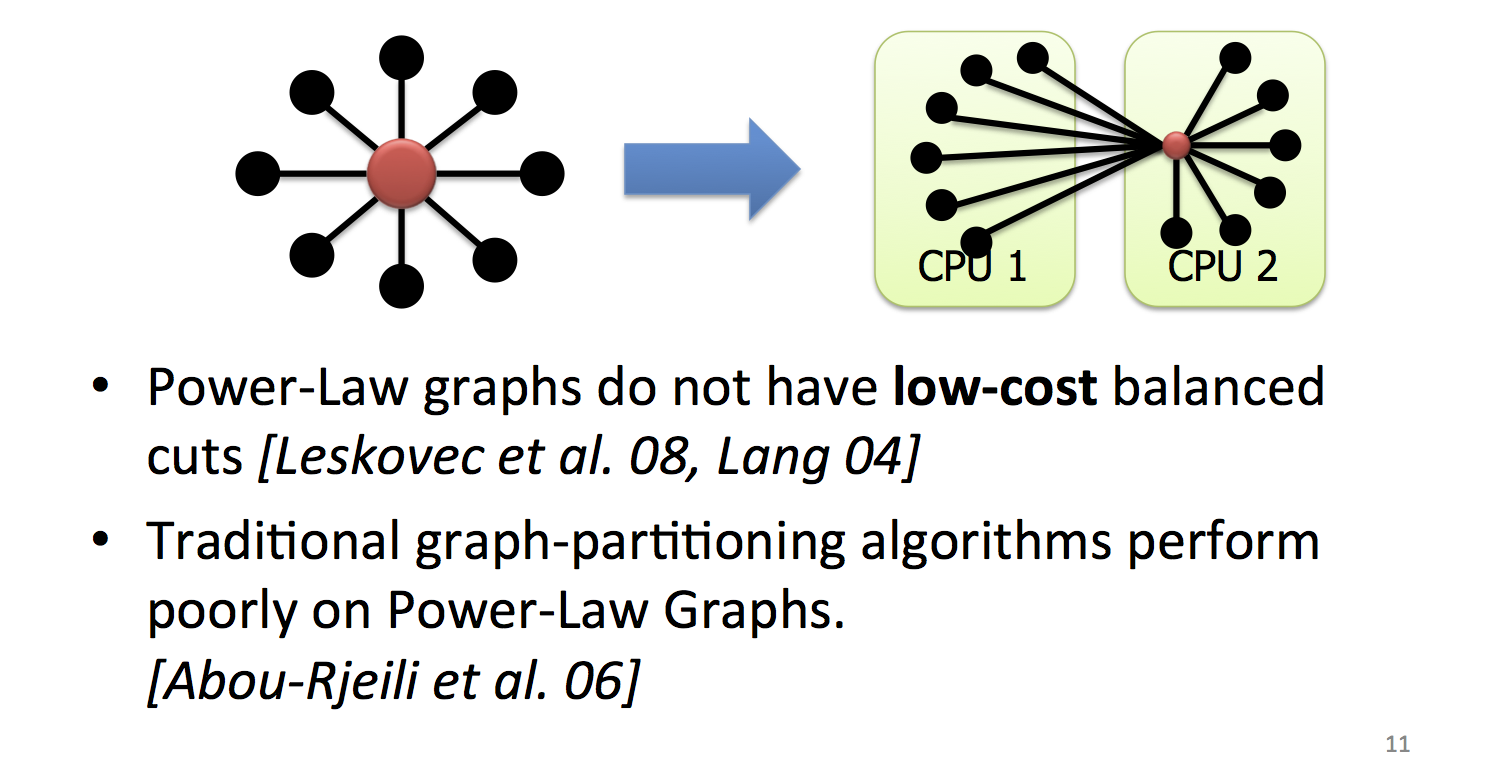
\includegraphics[scale=0.30]{gonzalez_osdi_2012_slide_11}
    \caption{\cite[OSDI '12 Slides]{gonzalez2012powergraph-slides}}
  \end{figure}
\end{frame}


\subsection{Some Background on Graph-Parallel Abstractions}

\begin{frame}
  \frametitle{Graph-Parallel Abstractions (A Review)}
  ``A graph parallel abstraction consists of a \textit{sparse} graph
  $G = \{V,E\}$ and a vertex-program $Q$ which is executed in parallel on each
  vertex $v \in V$ and can interact\ldots with neighboring
  instances.''\footnote{\cite[OSDI '12]{gonzalez2012powergraph}}


\end{frame}

\begin{frame}
  \frametitle{Graph-Parallel Abstractions (A Review)}
  ``In contrast to more general message passing models, graph-parallel
  abstractions constrain the interaction of vertex-program (sic) to a graph
  structure enabling the optimzation of data-layout and
  communication.''\footnote{\cite[OSDI '12]{gonzalez2012powergraph}}
\end{frame}

\begin{frame}
  \frametitle{Graph-Parallel Abstractions Used For Comparison}
  User-defined vertex programs run in parallel on many nodes:
  \begin{itemize}
    \item \textbf{Pregel:}\footnote{\cite[SIGMOD '10]{malewicz2010pregel}}
      \begin{itemize}
        \item Programs communicate via message passing along graph.
        \item Programs can change graph topology.
        \item Vertices own their state and state of their outgoing edges.
        \item Consistency via supersteps using a master node.
      \end{itemize}
    \item \textbf{GraphLab:}\footnote{\cite[VLDB '12]{low2012distributed}}
      \begin{itemize}
        \item Programs read/write shared data on a distributed graph.
        \item Graph topology is fixed.
        \item Good concurrency via smart scheduling of programs.
        \item Serializability via locking and inter-node messages.
      \end{itemize}
  \end{itemize}
\end{frame}


\subsection{The Challenges of Processing Power Law Graphs}

\begin{frame}
  \begin{figure}
    \centering
    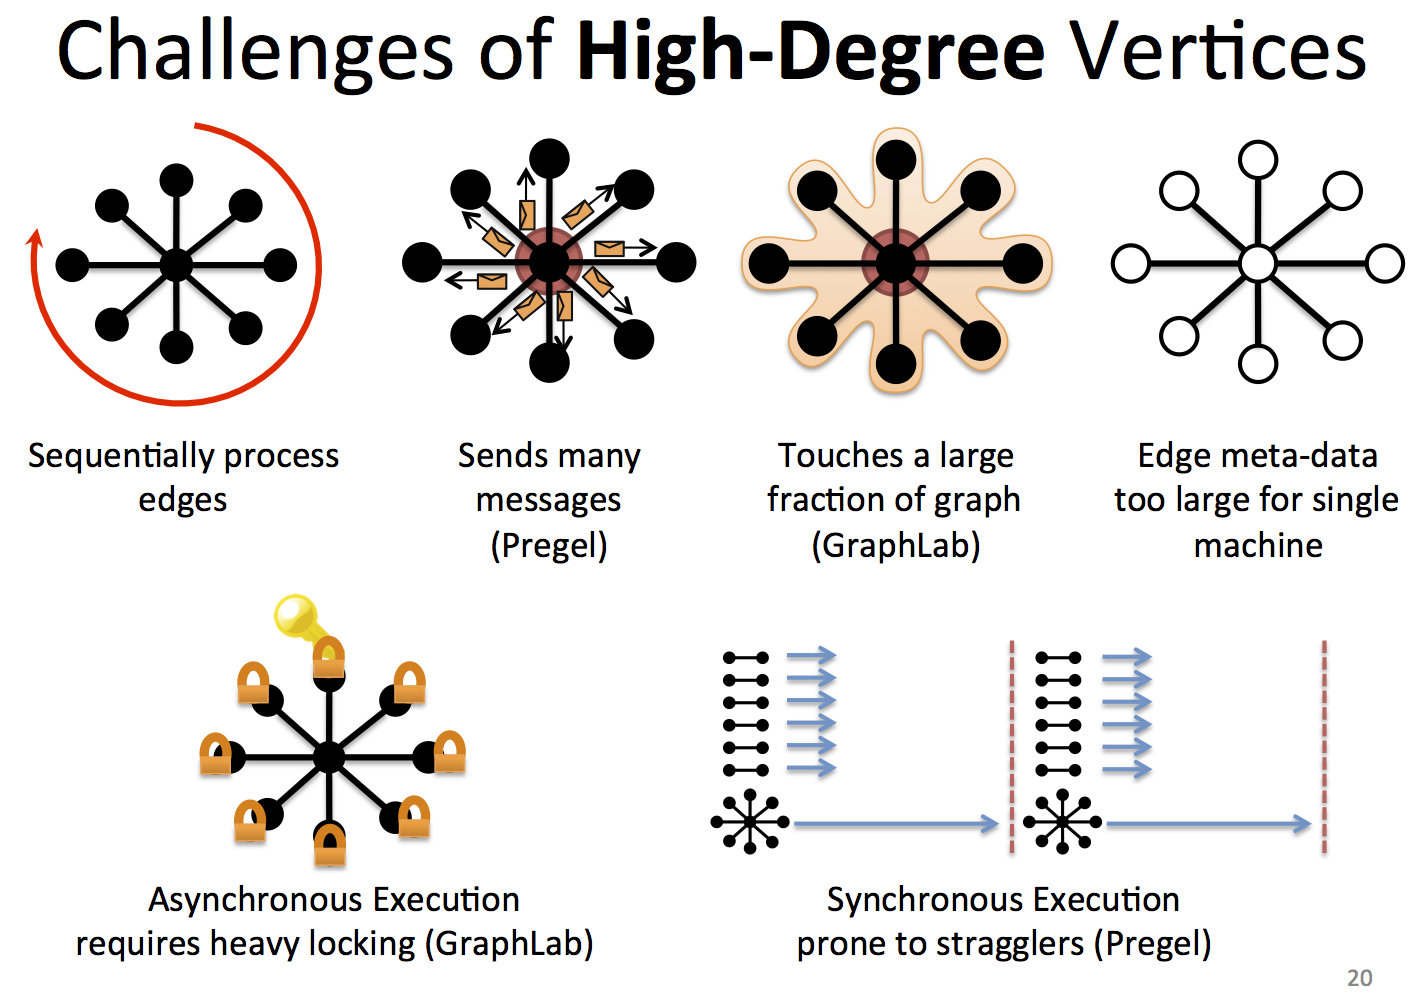
\includegraphics[scale=0.35]{gonzalez_osdi_2012_slide_20}
    \caption{\cite[OSDI '12]{gonzalez2012powergraph-slides}}
  \end{figure}
\end{frame}

\begin{frame}
  \frametitle{Challenges}
  The authors identify five ways in which these these properties of power law
  graphs create challenges for optimizations within pre-existing graph parallel
  abstractions:
  \begin{itemize}
    \item Work Balance
    \item Partitioning
    \item Communication
    \item Storage
    \item Computation
  \end{itemize}
\end{frame}
